\documentclass[11pt]{article}

\usepackage[margin=1in]{geometry}
\usepackage{amsmath,amssymb,amsthm}
\usepackage{graphicx}
\usepackage{booktabs}
\usepackage{caption}
\usepackage{natbib}
\usepackage{xcolor}
\usepackage[colorlinks=true,linkcolor=blue!50!black,citecolor=blue!50!black,urlcolor=blue!50!black]{hyperref}
\usepackage{enumitem}

\graphicspath{{../figures/}}
\bibliographystyle{plainnat}

\newtheorem{proposition}{Proposition}
\newtheorem{corollary}{Corollary}
\newtheorem{definition}{Definition}

\title{\textbf{Accelerant, Not Arsonist:}\\[2pt]
\large Latent--Demand Revelation and the Welfare Effects of Digital Asset Boards}

\author{}
\date{June 2026}

\begin{document}
\maketitle

\begin{abstract}
\noindent
Digital ``asset boards''---Zillow and Redfin for housing, LinkedIn and Indeed for jobs---are
popularly blamed for making life-changing assets scarcer and more expensive. I formalize and
test the strongest version of this claim, the \emph{latent-demand-revelation} hypothesis: by
aggregating buyers who were previously dispersed across segmented local markets, a board raises
the effective number of bidders per listing and bids up the price of a fixed stock. I show the
mechanism has a rigorous home in auction theory and market-integration theory---but \emph{not} in
the economics of search costs, where lower frictions have ambiguous and often price-reducing
effects. I then build an equilibrium assignment-market simulation that prices a fixed housing
stock via a forward-auction mechanism with individual rationality, and decompose the board's
effect into allocative efficiency versus surplus redistribution. The central result is a
\textbf{sign change at the scarcity threshold}: when supply is ample (buyers/homes $<1$) the board
\emph{lowers} prices and raises buyer surplus by 90--110\%; when supply binds (buyers/homes $>1$)
the same technology \emph{raises} prices by 33--63\% and transfers 17--50\% of buyer surplus to
sellers, while always achieving first-best allocative efficiency. Time-series evidence from U.S.
housing and labor markets is inconsistent with a platform-driven price break---Zillow launched at
the exact 2006 real-price peak, after which real prices fell $\approx$35\%---and points instead to
inelastic supply (housing) and labor demand (jobs) as the binding constraints. The platform is
best understood as an accelerant that capitalizes pre-existing scarcity into price and redistributes
the resulting rents toward sellers, not as a creator of scarcity. The price effect changes sign with
\emph{supply}, not with the platform; the policy lever is supply.

\medskip
\noindent\textbf{Keywords:} platform economics, search frictions, assignment games, housing supply,
labor matching, market design. \quad \textbf{JEL:} D44, D83, L86, R31, J64.
\end{abstract}

\section{Introduction}

A recurring popular argument holds that platforms aggregating high-stakes assets onto a single
searchable board---Zillow, Redfin and Realtor.com for homes; LinkedIn and Indeed for jobs---have
made those assets scarcer and more expensive, to the detriment of consumers. The proposed channel,
which I call \emph{latent-demand revelation}, is intuitive: before these platforms, demand for any
given home or job was dispersed across many thin, locally segmented markets; by pooling that demand
into one thick market, the board surfaces previously hidden competition, raises the number of
bidders contesting each listing, and bids up the equilibrium price of a stock that the platform
itself cannot expand.

This paper takes the hypothesis seriously and subjects it to theory, simulation, and data. Three
questions organize the analysis. First, does the mechanism have a coherent theoretical foundation,
and if so which one? Second, if we hold physical supply fixed and aggregate demand, what happens to
the \emph{level} of prices and to the \emph{distribution} of surplus between buyers and sellers?
Third, is the mechanism quantitatively important relative to the leading competing explanation---that
the binding constraint is inelastic supply, with the platform merely a visibility layer on top of
pre-existing scarcity?

My answers are, respectively: yes but with a crucial caveat about which theory applies; the effect
depends entirely on whether supply binds; and the competing explanation dominates the \emph{level}
of prices while the platform mechanism operates at the \emph{margin} and on the \emph{distribution}.
The strong form of the hypothesis---that platforms \emph{cause} scarcity---is false, because a
listing board cannot reduce the physical stock of homes or the number of jobs. The weak, conditional
form is correct and is the analytically interesting result: latent-demand revelation converts
pre-existing scarcity into higher transaction prices and a buyer-to-seller surplus transfer, but
only when supply is already the binding constraint.

\section{The mechanism: an auction story, not a search-cost story}\label{sec:mech}

It is essential to identify \emph{which} body of theory rationalizes latent-demand revelation,
because two candidate theories make opposite predictions.

\paragraph{The correct foundation: order statistics.}
Consider a single unique asset sold to the highest of $n$ bidders with independent private
valuations. In a second-price (or competitive ascending) auction the sale price equals the
second-highest valuation, whose expectation is increasing in $n$.

\begin{proposition}[Demand aggregation raises price for fixed supply]\label{prop:os}
Let $n$ bidders have i.i.d.\ private valuations with continuous c.d.f.\ $F$. The expected
competitive sale price $\mathbb{E}[V_{(n-1:n)}]$, the second-highest order statistic, is
strictly increasing in $n$. For the uniform case $F=U[0,1]$,
\[
\mathbb{E}\big[V_{(n-1:n)}\big] \;=\; \frac{n-1}{n+1},
\]
which rises from $\tfrac13$ at $n=2$ toward $1$ as $n\to\infty$.
\end{proposition}

\noindent The proof is the standard order-statistic computation \citep{easleykleinberg2010}; by the
Revenue Equivalence Theorem the comparative static ``more bidders $\Rightarrow$ higher expected
revenue'' extends across standard auction formats \citep{vickrey1961,rileysamuelson1981,myerson1981}.
Aggregating buyers from $S$ segmented submarkets onto one board is formally equivalent to enlarging
the bidder pool contesting each listing. Market-integration theory delivers the same conclusion from
a different direction: integrating segmented markets raises prices in the formerly cheap ``surplus''
region as the law of one price asserts itself.

\paragraph{The wrong foundation: search costs.}
A tempting but incorrect version of the hypothesis is ``boards lower search costs, which raises
prices.'' Search theory predicts no such monotone relationship. In the Diamond paradox
\citep{diamond1971}, driving search costs toward zero pushes the equilibrium toward the competitive
price; the pathological monopoly outcome occurs for \emph{positive} search costs, and the
discontinuity is precisely at zero. Welfare and price effects of search frictions are formally
ambiguous, pinned down only by the knife-edge efficiency condition of \citet{hosios1990}, and
\citet{bakos1997} shows that lower buyer search costs \emph{reduce} sellers' market power in
differentiated-product markets. \citet{stahl1989} provides a model in which lower search costs and
more sellers \emph{raise} prices, but through oligopolistic price dispersion, not demand pooling.

\begin{corollary}
The defensible form of the latent-demand-revelation hypothesis runs through demand \emph{pooling}
(bidder-pool enlargement against fixed supply), not through reduced search costs in general.
\end{corollary}

\section{An equilibrium model of aggregation under fixed supply}\label{sec:model}

\subsection{Environment}
There are $H$ indivisible homes (fixed supply) and $B$ buyers with unit demand. Buyer $i$'s
valuation for home $j$ is
\begin{equation}
a_{ij} \;=\; q_j \;+\; \kappa\, m_{ij},
\end{equation}
where $q_j\ge 0$ is a common \emph{vertical} quality (all buyers agree San Francisco $\succ$ Fresno)
and $m_{ij}\ge 0$ is an idiosyncratic \emph{horizontal} match (one buyer prefers a loft, another a
craftsman). The parameter $\kappa$ scales the importance of taste heterogeneity and hence the size
of the sorting gains available from better matching. Buyers have an outside option normalized to $0$.

Two information regimes differ only in \emph{visibility}:
\begin{description}[leftmargin=2em,itemsep=1pt]
\item[Segmented.] The market is partitioned into $S$ ``islands.'' Buyer $i$ can transact only with
homes on her island. This is the pre-platform world of dispersed local markets.
\item[Board.] Every buyer can transact with every home---the Zillow world.
\end{description}
Crucially, $H$ is identical across regimes: \emph{the platform changes who can see what, never how
many homes exist}. Market tightness is $\theta \equiv B/H$.

\subsection{Equilibrium concept and pricing}
The economy is an assignment game \citep{shapleyshubik1971}. A competitive equilibrium is a price
vector $p\in\mathbb{R}^H_+$ and an assignment $\mu$ such that (i) each buyer is matched to a home in
her demand set $\arg\max_j\{a_{ij}-p_j,\,0\}$, and (ii) markets clear. The set of equilibrium prices
forms a lattice; we compute the buyer-optimal (minimal) equilibrium using Bertsekas's forward-auction
algorithm \citep{bertsekas1988} augmented with the individual-rationality constraint that no buyer
bids above her valuation. The algorithm has a transparent economic interpretation---buyers
iteratively bid for their most profitable home, raising its price by their net-value advantage over
their next-best option plus an increment $\varepsilon$---and converges to an assignment within
$H\varepsilon$ of efficiency with prices accurate to $\varepsilon$.

\subsection{What to expect}
Because the board's feasible matches are a superset of the segmented regime's, the board weakly
raises realized total surplus (better sorting), so \emph{allocative efficiency rises
unambiguously}. The effect on the \emph{price level} is the open question. With slack supply
($\theta<1$) homes compete for buyers, and widening each buyer's choice set should intensify
competition \emph{among sellers}, lowering prices. With binding supply ($\theta>1$) buyers compete
for homes, and revealing the latent pool of rival bidders should raise the marginal clearing
valuation, i.e.\ Proposition~\ref{prop:os} operating in general equilibrium. The simulation
quantifies where the crossover lies.

\section{Simulation results}\label{sec:sim}

I set $H=60$, $S=6$, $\kappa=0.8$, with $q_j$ lognormal (mean 1) and $m_{ij}$ Gamma (mean 1), and
sweep $\theta\in\{0.8,1.0,1.25,1.5,2.0\}$, averaging over 20 independent markets per cell. Code is in
\texttt{code/01\_simulation.py}.

\subsection{Experiment A: a single scarce asset}
Figure~\ref{fig:os} confirms Proposition~\ref{prop:os} under realistic (lognormal) valuations and
shows steeply diminishing returns to revealed bidders. Going from a thin local pool to a thick
national one raises the expected sale price substantially: $n{:}\,3\to15$ yields $+81\%$ and
$3\to30$ yields $+116\%$ (normalizing mean willingness-to-pay to 1). The convexity matters
substantively: \emph{thin, previously-segmented markets are exactly where revelation bites hardest}.

\begin{figure}[t]
\centering
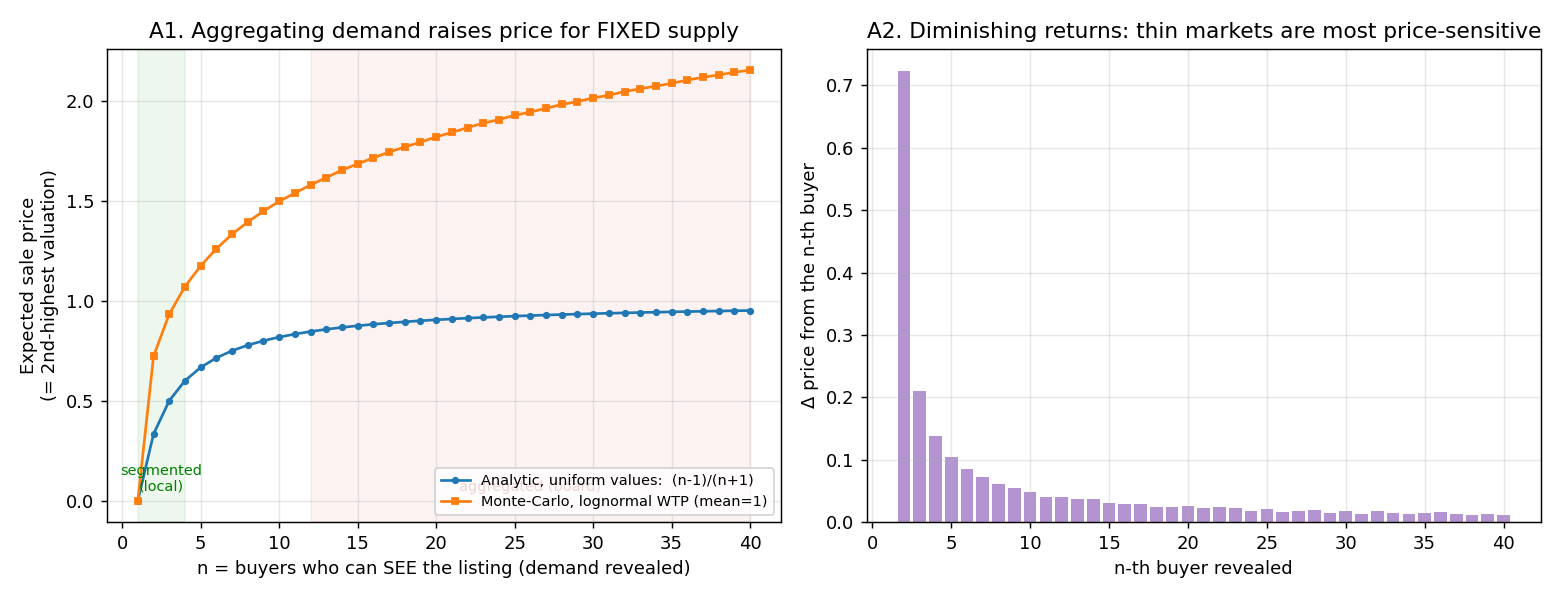
\includegraphics[width=\textwidth]{fig1_order_statistics.png}
\caption{Expected sale price (= second-highest valuation) versus the number of buyers who can see a
listing. Left: analytic uniform benchmark $(n{-}1)/(n{+}1)$ and Monte-Carlo with lognormal
willingness-to-pay. Right: marginal price contribution of the $n$-th revealed bidder.}
\label{fig:os}
\end{figure}

\subsection{Experiment B: the equilibrium decomposition}
Table~\ref{tab:sim} and Figure~\ref{fig:decomp} report the board-versus-segmented comparison.

\begin{table}[t]
\centering
\caption{Board vs.\ segmented market, by tightness $\theta=B/H$ (percentage changes; means over 20 runs).}
\label{tab:sim}
\begin{tabular}{lccccc}
\toprule
$\theta$ & Avg.\ price & Total surplus & Buyer surplus & Seller revenue & Efficiency (seg $\to$ board) \\
\midrule
0.8 (ample)   & $-40\%$ & $+39\%$ & $+93\%$  & $-34\%$ & $0.72 \to 1.00$ \\
1.0 (balanced)& $-24\%$ & $+46\%$ & $+113\%$ & $-10\%$ & $0.68 \to 1.00$ \\
1.25 (tight)  & $+63\%$ & $+39\%$ & $-45\%$  & $+78\%$ & $0.72 \to 1.00$ \\
1.5 (scarce)  & $+52\%$ & $+32\%$ & $-50\%$  & $+57\%$ & $0.75 \to 1.00$ \\
2.0 (acute)   & $+33\%$ & $+28\%$ & $-17\%$  & $+33\%$ & $0.79 \to 1.00$ \\
\bottomrule
\end{tabular}
\end{table}

\begin{figure}[t]
\centering
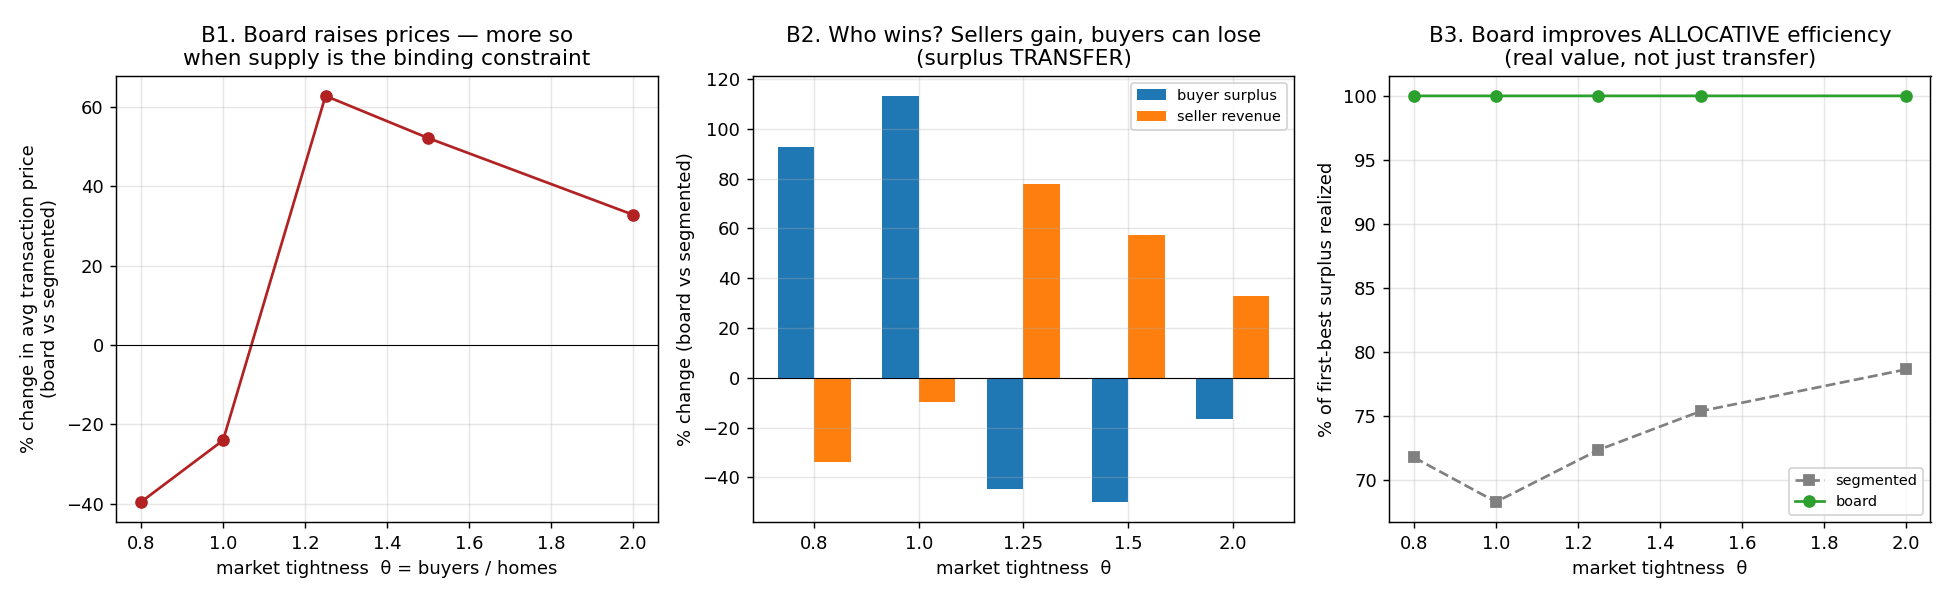
\includegraphics[width=\textwidth]{fig2_assignment_decomposition.png}
\caption{Decomposition of the board's effect. Left: change in average transaction price crosses zero
at the scarcity threshold $\theta\approx1$. Center: buyer-surplus and seller-revenue changes are
mirror images---a redistribution. Right: the board achieves first-best allocative efficiency at all
$\theta$, while the segmented market realizes only 68--79\%.}
\label{fig:decomp}
\end{figure}

Three findings emerge.

\begin{enumerate}[leftmargin=1.6em,itemsep=2pt]
\item \textbf{Sign change at $\theta\approx1$.} When homes are not scarce, aggregation lowers prices
and sharply raises buyer surplus---the optimistic \citet{browngoolsbee2002}/\citet{bakos1997}
result. When homes are scarce, the \emph{same} technology raises prices 33--63\% and destroys
17--50\% of buyer surplus. The platform did not change; the supply condition did. This is the precise
sense in which the popular hypothesis is true: \emph{latent-demand revelation hurts consumers if and
only if supply is the binding constraint}.
\item \textbf{Redistribution, not destruction.} Where buyers lose, sellers gain by roughly the same
amount and total surplus still rises. The harm is distributional---thick-market competition hands the
gains from trade to the scarce side.
\item \textbf{Efficiency always improves.} The board sorts each asset to its highest-value user,
reaching first best ($1.00$ vs.\ $0.68$--$0.79$). Any honest critique of the platforms must concede
this productivity gain; the debate is about the price level and distribution, not waste.
\end{enumerate}

\section{Empirical evidence}\label{sec:emp}

The model says the hypothesis requires binding supply ($\theta>1$). The aggregate U.S. data say that
condition---not the platforms---is what moved. Series are drawn from FRED; code is in
\texttt{code/02\_empirics.py}.

\paragraph{Housing timing contradicts a platform price break.}
Figure~\ref{fig:housing} shows real Case--Shiller prices. Zillow and Redfin both launched in
February 2006, the \emph{exact} peak of real prices, after which real prices fell roughly 35\% to
their 2012 trough \emph{while platform adoption exploded}. The post-2012 recovery and 2020--22 spike
track interest rates, a pandemic demand shock, and a supply freeze---not a platform that was already
mature by 2012. The real price-to-income ratio peaked near 2006 ($5.3\times$) and 2022 ($5.9\times$);
today's $5.0\times$ is below its 2006 level.

\begin{figure}[t]
\centering
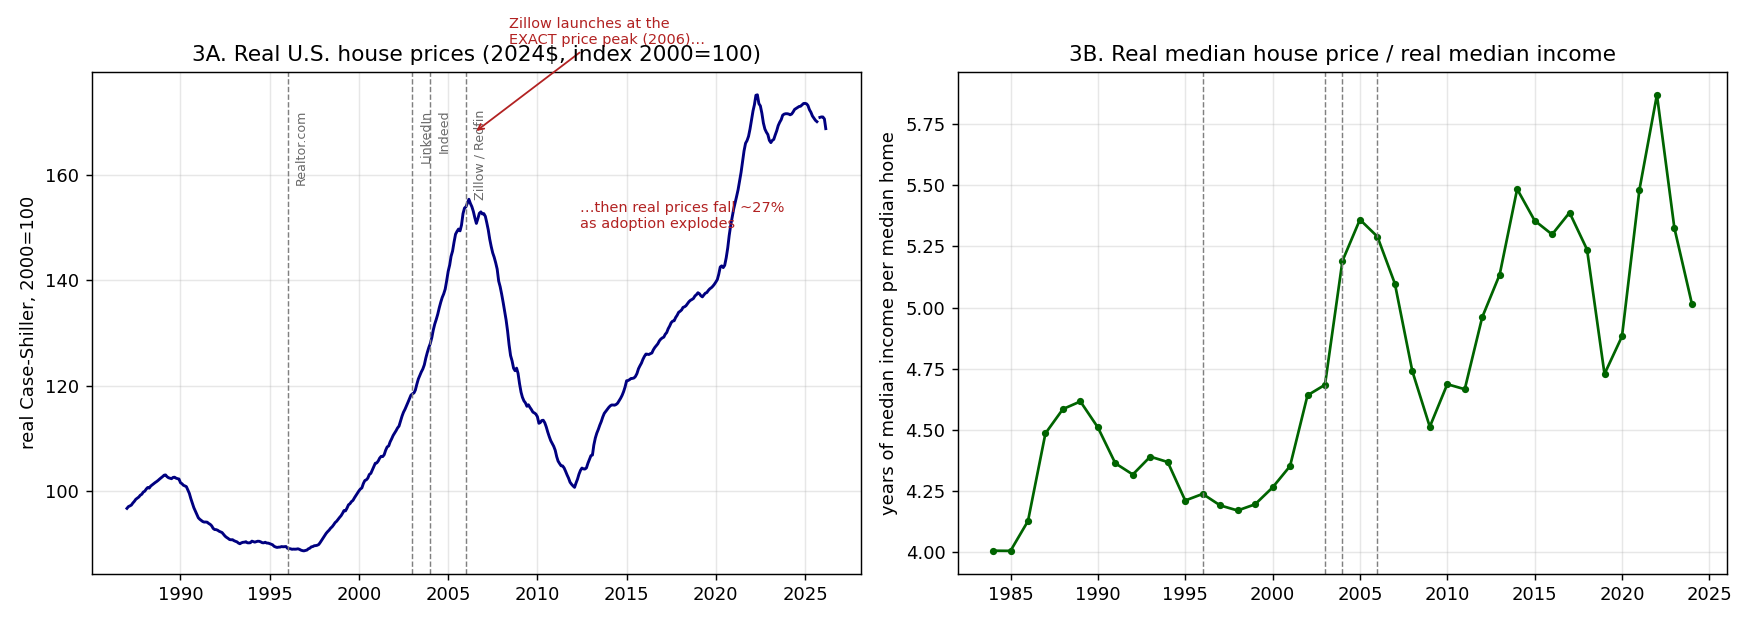
\includegraphics[width=\textwidth]{fig3_housing_timeline.png}
\caption{Real U.S.\ house prices (left) and real price-to-income (right), with platform launch dates.
Zillow/Redfin launched at the 2006 real-price peak; prices then fell as adoption rose.}
\label{fig:housing}
\end{figure}

\paragraph{Recent scarcity is a supply-side inventory story.}
Figure~\ref{fig:inv} shows active for-sale listings falling $\approx$28\% from 2016 to 2026,
collapsing in 2020--22 from the demand shock plus mortgage-rate ``lock-in'' freezing supply. This is
$\theta$ rising for reasons unrelated to the platforms' existence (which predate the collapse by a
decade), and it is precisely the regime in which the model predicts the platform channel pushes prices
up---as an accelerant of supply-driven scarcity.

\begin{figure}[t]
\centering
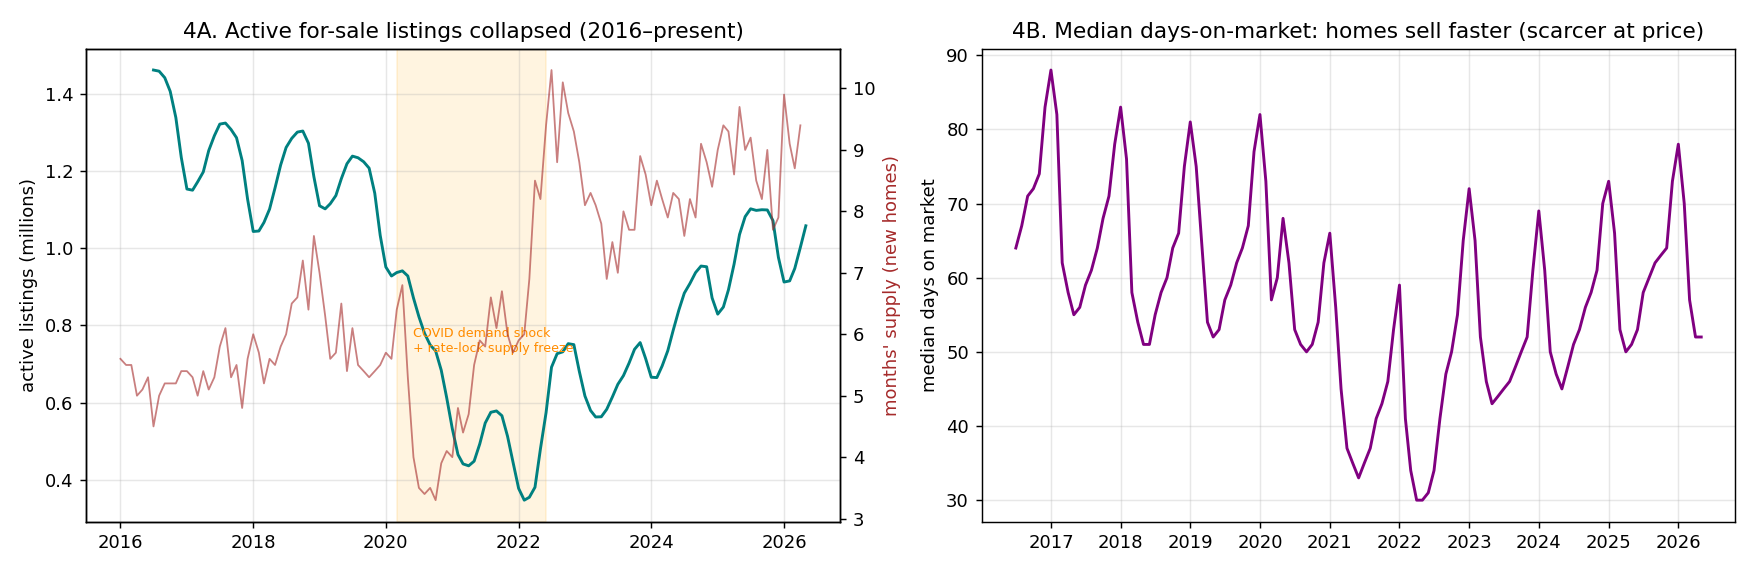
\includegraphics[width=\textwidth]{fig4_inventory.png}
\caption{Active listings and months' supply (left) and median days-on-market (right), 2016--present.}
\label{fig:inv}
\end{figure}

\paragraph{Labor: matching did not break and wages did not fall.}
Figure~\ref{fig:labor} shows the Beveridge curve's well-documented post-2009 and pandemic outward
shifts---attributed in the literature to sectoral mismatch and benefits, not to job boards---and real
median weekly earnings rising $\approx$12\% since LinkedIn's 2003 founding. The cleanest causal
studies point the pro-worker way: exogenous broadband expansion cut vacancy durations and raised
job-finding rates and starting wages \citep{bhuller2022}; online search reemployed workers faster
\citep{kuhnmansour2014}; and LinkedIn ``weak ties'' causally raise job mobility in a 20-million-user
randomized experiment \citep{rajkumar2022}. \citet{kroftpope2014} find Craigslist's entry reduced
rental vacancies and time-to-lease without changing the housing stock and had no effect on aggregate
unemployment---frictions, not quantities.

\begin{figure}[t]
\centering
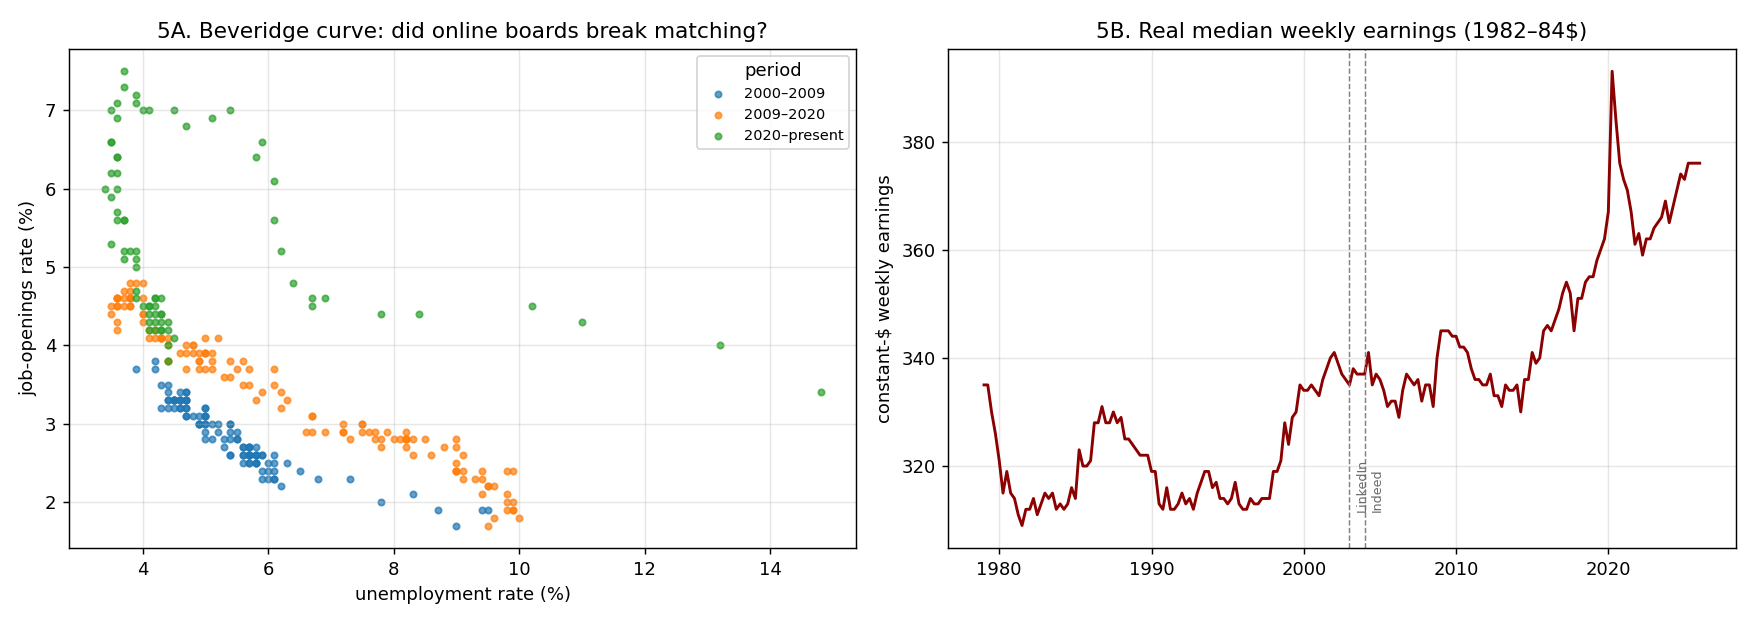
\includegraphics[width=\textwidth]{fig5_labor.png}
\caption{Beveridge curve by period (left) and real median weekly earnings (right).}
\label{fig:labor}
\end{figure}

\section{Discussion: where the platform-blame story does and does not hold}

The supply-inelasticity literature is decisive about price \emph{levels}. Expensive housing is
geographically concentrated in supply-constrained metros, with the wedge between price and
construction cost ranging from near zero in elastic markets to roughly half the price in the most
regulated ones \citep{saiz2010,glaesergyourko2005,gyourkomolloy2015}. A national platform cannot
explain a local price pattern, and with fixed supply better search mainly \emph{reallocates} the
scarce asset \citep{kroftpope2014}. The induced-demand analogue from transportation---capacity
expansions absorbed by latent demand \citep{durantonturner2011}---reinforces that revealing listings
mobilizes latent buyers who keep competition tight.

Where the platform-blame story retains force is exactly the model's $\theta>1$ region, plus two
amplifiers the literature documents as genuinely price-raising---and, tellingly, neither is
``search'' per se. First, \emph{seller-side coordination}: transparency among sellers can support
collusion \citep{albaek1997,schultz2005}, whose sharpest modern form is algorithmic rent-setting
\citep{doj2024realpage,cea2024}. Second, \emph{demand concentration}: superstar dynamics
\citep{rosen1981,autor2020} let boards concentrate demand on top assets and candidates, widening
dispersion. Notably, Zillow's own iBuying collapse---a half-billion-dollar write-down and program
exit in 2021---demonstrates that its algorithms cannot reliably predict, let alone control, home
prices \citep{ibuyers2021}, undercutting the strongest ``platforms set prices'' intuition.

\section{Conclusion}

Asset boards are accelerants, not arsonists. They cannot create physical scarcity; the binding
constraints are inelastic housing supply and labor demand. But in a supply-constrained market,
latent-demand revelation---an auction/order-statistic mechanism, not a search-cost one---capitalizes
that scarcity more fully into price and hands the surplus to the scarce side, while simultaneously
improving allocative efficiency and, in slack markets, \emph{helping} buyers. The consumer-welfare
effect of these platforms changes sign with the supply condition, not with the platform. The policy
implication follows directly: the lever that flips the sign is supply---build housing and expand the
stock of good jobs to push $\theta$ below one---while the narrow, genuinely regulatable platform harms
are algorithmic seller coordination and demand-concentrating practices, not searchability itself.

\paragraph{Caveats.}
The simulation is an illustrative calibration, not an estimated structural model; it establishes the
mechanism's direction, sign change, and rough magnitude, not field-validated elasticities. The
time-series evidence is descriptive: it shows the aggregate facts are inconsistent with a simple
platform-driven price break, not a causal platform treatment effect. Several cited empirical
magnitudes (e.g.\ algorithmic-pricing rent overcharges, aggregate misallocation costs) are
associational or contested and are flagged as such in the accompanying source register.

\bibliography{refs}

\end{document}
